% Shared preamble for the English summaries in this repository.
\documentclass[11pt,a4paper]{article}
\usepackage[margin=2.2cm]{geometry}
\usepackage[T1]{fontenc}
\usepackage[utf8]{inputenc}
\usepackage{lmodern}
\usepackage{amsmath,amssymb}
\usepackage{graphicx}
\usepackage{booktabs}
\usepackage{enumitem}
\usepackage[hidelinks]{hyperref}
\setlist{itemsep=2pt,topsep=4pt}
\setlength{\parindent}{0pt}
\setlength{\parskip}{5pt}
\graphicspath{{figures/}}
\newcommand{\summaryheader}[3]{%
  \begin{center}
    {\Large\bfseries #2}\\[3pt]
    {\large #1}\\[3pt]
    {\small Arshia Goshtasbi \textbullet{} MSc Electrical Engineering (Control), Iran University of Science and Technology \textbullet{} #3}
  \end{center}
  \vspace{2pt}\hrule\vspace{8pt}\par}

\begin{document}
\summaryheader{Machine Learning, Homework 5}{Support Vector Machines from a QP Solver and with Kernels}{Spring 1404 (2025)}

\textbf{Notebook} (\texttt{svm.ipynb}). The data are Statlog (Landsat) satimage: 36 features, 6 classes. I used a stratified 60/15/25 split and standardised the features.
\begin{itemize}
  \item \emph{Soft-margin SVM from scratch.} I wrote the dual QP in the standard form $\min\tfrac12\alpha^\top P\alpha+q^\top\alpha$ subject to $G\alpha\le h$ and $A\alpha=b$, and solved it with \texttt{cvxopt}. Then I recovered $w$ and $b$ from the support vectors. The binary task uses classes 4 and 5 (the notebook text says 4 and 6; the code uses 4 and 5). With $C=1$ the linear model reaches accuracy $0.961$ and balanced accuracy $0.961$ on the test set.
  \item \emph{RBF kernel, also from scratch.} I picked $\gamma$ on the validation set by balanced accuracy. The best was $\gamma=0.001$, which gives test accuracy $0.904$, lower than the linear model.
  \item \emph{Multiclass} \texttt{SVC} with an RBF kernel and a grid search over $C$ and $\gamma$: best $C=10$, $\gamma=0.1$, with accuracy $0.929$ and balanced accuracy $0.902$. Most errors are between classes 3, 4 and 6 (Figure~\ref{fig:svm}).
  \item \emph{Kernel comparison} with default settings: linear $0.866$, RBF $0.914$, polynomial (degree 3) $0.873$, sigmoid $0.716$ accuracy.
  \item An optional multiclass SVM trained by sub-gradient descent from scratch reached only $0.46$.
\end{itemize}

\begin{figure}[h]\centering
  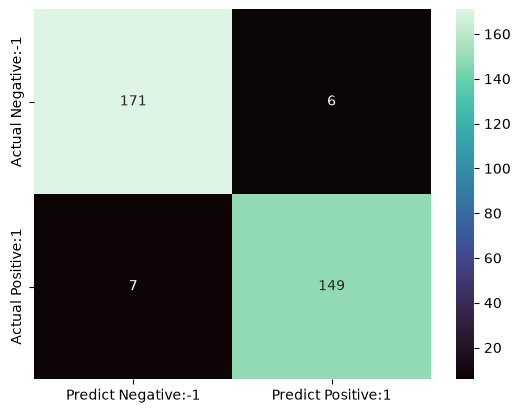
\includegraphics[width=.42\linewidth]{svm_cell21_1.png}\hspace{1em}
  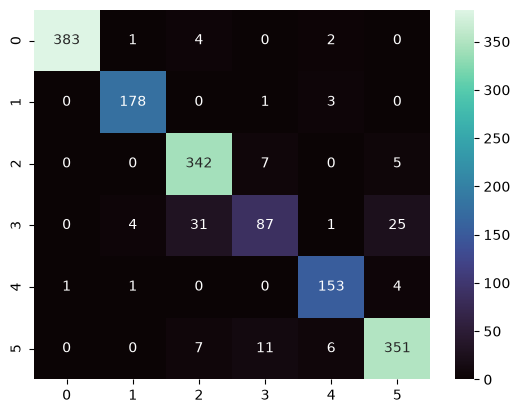
\includegraphics[width=.42\linewidth]{svm_cell30_1.png}
  \caption{Confusion matrices: from-scratch linear SVM, classes 4 vs.\ 5 (left); tuned multiclass RBF SVC (right).}\label{fig:svm}
\end{figure}

\textbf{Written part.}
\begin{description}
  \item[$L_2$ soft-margin SVM.] The constraint $\xi_i\ge0$ can be dropped: a negative $\xi_i$ only increases $\xi_i^2$ and is never needed to satisfy the margin, so the optimum is unchanged. I wrote the Lagrangian and minimised it over $w$, $b$ and $\xi$ ($w=\sum\alpha_iy_ix_i$, $\sum\alpha_iy_i=0$, $\xi=\alpha/C$). The dual is $\max_{\alpha\ge0}\sum\alpha_i-\tfrac12\sum_{ij}\alpha_i\alpha_jy_iy_j\big(x_i^\top x_j+\delta_{ij}/C\big)$ with $\sum\alpha_iy_i=0$.
  \item[Two points with a quadratic feature map.] For $\phi(x)=[1,\sqrt2x,x^2]$, $x_1=0$, $x_2=\sqrt2$, the optimal $w$ is parallel to $\phi(x_2)-\phi(x_1)=(0,2,2)$. The margin is half the distance between the mapped points, $\sqrt2$, so $w=(0,\tfrac12,\tfrac12)$.
  \item[Kernel closure.] Positive scaling, sums and products of valid kernels are valid kernels (the Gram matrices stay positive semidefinite; for the product, use the Schur product theorem).
\end{description}
\end{document}
